\documentclass[]{article}
\usepackage{lmodern}
\usepackage{amssymb,amsmath}
\usepackage{ifxetex,ifluatex}
\usepackage{fixltx2e} % provides \textsubscript
\ifnum 0\ifxetex 1\fi\ifluatex 1\fi=0 % if pdftex
  \usepackage[T1]{fontenc}
  \usepackage[utf8]{inputenc}
\else % if luatex or xelatex
  \ifxetex
    \usepackage{mathspec}
  \else
    \usepackage{fontspec}
  \fi
  \defaultfontfeatures{Ligatures=TeX,Scale=MatchLowercase}
  \newcommand{\euro}{€}
\fi
% use upquote if available, for straight quotes in verbatim environments
\IfFileExists{upquote.sty}{\usepackage{upquote}}{}
% use microtype if available
\IfFileExists{microtype.sty}{%
\usepackage{microtype}
\UseMicrotypeSet[protrusion]{basicmath} % disable protrusion for tt fonts
}{}
\usepackage[margin=1in]{geometry}
\usepackage{hyperref}
\PassOptionsToPackage{usenames,dvipsnames}{color} % color is loaded by hyperref
\hypersetup{unicode=true,
            pdftitle={Lecture 05:Data visualization and graphics in R},
            pdfborder={0 0 0},
            breaklinks=true}
\urlstyle{same}  % don't use monospace font for urls
\usepackage{color}
\usepackage{fancyvrb}
\newcommand{\VerbBar}{|}
\newcommand{\VERB}{\Verb[commandchars=\\\{\}]}
\DefineVerbatimEnvironment{Highlighting}{Verbatim}{commandchars=\\\{\}}
% Add ',fontsize=\small' for more characters per line
\usepackage{framed}
\definecolor{shadecolor}{RGB}{248,248,248}
\newenvironment{Shaded}{\begin{snugshade}}{\end{snugshade}}
\newcommand{\KeywordTok}[1]{\textcolor[rgb]{0.13,0.29,0.53}{\textbf{{#1}}}}
\newcommand{\DataTypeTok}[1]{\textcolor[rgb]{0.13,0.29,0.53}{{#1}}}
\newcommand{\DecValTok}[1]{\textcolor[rgb]{0.00,0.00,0.81}{{#1}}}
\newcommand{\BaseNTok}[1]{\textcolor[rgb]{0.00,0.00,0.81}{{#1}}}
\newcommand{\FloatTok}[1]{\textcolor[rgb]{0.00,0.00,0.81}{{#1}}}
\newcommand{\ConstantTok}[1]{\textcolor[rgb]{0.00,0.00,0.00}{{#1}}}
\newcommand{\CharTok}[1]{\textcolor[rgb]{0.31,0.60,0.02}{{#1}}}
\newcommand{\SpecialCharTok}[1]{\textcolor[rgb]{0.00,0.00,0.00}{{#1}}}
\newcommand{\StringTok}[1]{\textcolor[rgb]{0.31,0.60,0.02}{{#1}}}
\newcommand{\VerbatimStringTok}[1]{\textcolor[rgb]{0.31,0.60,0.02}{{#1}}}
\newcommand{\SpecialStringTok}[1]{\textcolor[rgb]{0.31,0.60,0.02}{{#1}}}
\newcommand{\ImportTok}[1]{{#1}}
\newcommand{\CommentTok}[1]{\textcolor[rgb]{0.56,0.35,0.01}{\textit{{#1}}}}
\newcommand{\DocumentationTok}[1]{\textcolor[rgb]{0.56,0.35,0.01}{\textbf{\textit{{#1}}}}}
\newcommand{\AnnotationTok}[1]{\textcolor[rgb]{0.56,0.35,0.01}{\textbf{\textit{{#1}}}}}
\newcommand{\CommentVarTok}[1]{\textcolor[rgb]{0.56,0.35,0.01}{\textbf{\textit{{#1}}}}}
\newcommand{\OtherTok}[1]{\textcolor[rgb]{0.56,0.35,0.01}{{#1}}}
\newcommand{\FunctionTok}[1]{\textcolor[rgb]{0.00,0.00,0.00}{{#1}}}
\newcommand{\VariableTok}[1]{\textcolor[rgb]{0.00,0.00,0.00}{{#1}}}
\newcommand{\ControlFlowTok}[1]{\textcolor[rgb]{0.13,0.29,0.53}{\textbf{{#1}}}}
\newcommand{\OperatorTok}[1]{\textcolor[rgb]{0.81,0.36,0.00}{\textbf{{#1}}}}
\newcommand{\BuiltInTok}[1]{{#1}}
\newcommand{\ExtensionTok}[1]{{#1}}
\newcommand{\PreprocessorTok}[1]{\textcolor[rgb]{0.56,0.35,0.01}{\textit{{#1}}}}
\newcommand{\AttributeTok}[1]{\textcolor[rgb]{0.77,0.63,0.00}{{#1}}}
\newcommand{\RegionMarkerTok}[1]{{#1}}
\newcommand{\InformationTok}[1]{\textcolor[rgb]{0.56,0.35,0.01}{\textbf{\textit{{#1}}}}}
\newcommand{\WarningTok}[1]{\textcolor[rgb]{0.56,0.35,0.01}{\textbf{\textit{{#1}}}}}
\newcommand{\AlertTok}[1]{\textcolor[rgb]{0.94,0.16,0.16}{{#1}}}
\newcommand{\ErrorTok}[1]{\textcolor[rgb]{0.64,0.00,0.00}{\textbf{{#1}}}}
\newcommand{\NormalTok}[1]{{#1}}
\usepackage{graphicx,grffile}
\makeatletter
\def\maxwidth{\ifdim\Gin@nat@width>\linewidth\linewidth\else\Gin@nat@width\fi}
\def\maxheight{\ifdim\Gin@nat@height>\textheight\textheight\else\Gin@nat@height\fi}
\makeatother
% Scale images if necessary, so that they will not overflow the page
% margins by default, and it is still possible to overwrite the defaults
% using explicit options in \includegraphics[width, height, ...]{}
\setkeys{Gin}{width=\maxwidth,height=\maxheight,keepaspectratio}
\setlength{\parindent}{0pt}
\setlength{\parskip}{6pt plus 2pt minus 1pt}
\setlength{\emergencystretch}{3em}  % prevent overfull lines
\providecommand{\tightlist}{%
  \setlength{\itemsep}{0pt}\setlength{\parskip}{0pt}}
\setcounter{secnumdepth}{0}

\title{Lecture 05:Data visualization and graphics in R}
\author{}
\date{\vspace{-2.5em}}

% Redefines (sub)paragraphs to behave more like sections
\ifx\paragraph\undefined\else
\let\oldparagraph\paragraph
\renewcommand{\paragraph}[1]{\oldparagraph{#1}\mbox{}}
\fi
\ifx\subparagraph\undefined\else
\let\oldsubparagraph\subparagraph
\renewcommand{\subparagraph}[1]{\oldsubparagraph{#1}\mbox{}}
\fi

\begin{document}
\maketitle

\begin{Shaded}
\begin{Highlighting}[]
\KeywordTok{plot}\NormalTok{(}\DecValTok{1}\NormalTok{:}\DecValTok{5}\NormalTok{, }\DataTypeTok{col=}\StringTok{"blue"}\NormalTok{, }\DataTypeTok{typ=}\StringTok{"o"}\NormalTok{)}
\end{Highlighting}
\end{Shaded}

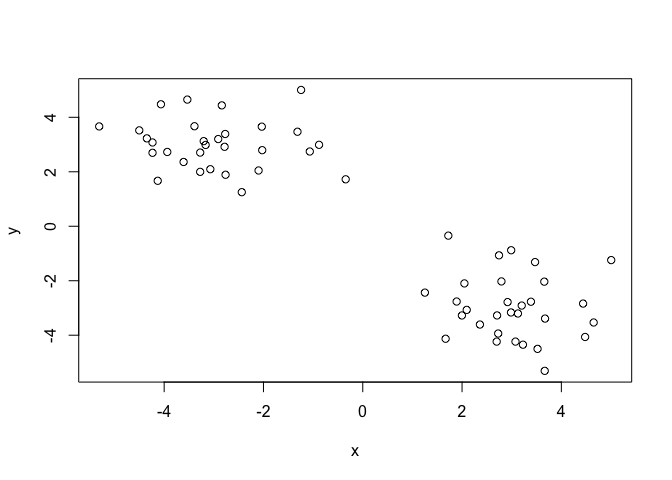
\includegraphics{class05_files/figure-latex/unnamed-chunk-1-1.pdf}

\begin{Shaded}
\begin{Highlighting}[]
\NormalTok{baby <-}\StringTok{ }\KeywordTok{read.table}\NormalTok{(}\StringTok{"bimm143_05_rstats/weight_chart.txt"}\NormalTok{)}
\end{Highlighting}
\end{Shaded}

\begin{Shaded}
\begin{Highlighting}[]
\KeywordTok{View}\NormalTok{(baby)}
\end{Highlighting}
\end{Shaded}

\begin{Shaded}
\begin{Highlighting}[]
\NormalTok{baby <-}\StringTok{ }\KeywordTok{read.table}\NormalTok{(}\StringTok{"bimm143_05_rstats/weight_chart.txt"}\NormalTok{, }
                   \DataTypeTok{header =} \OtherTok{TRUE}\NormalTok{)}
\end{Highlighting}
\end{Shaded}

\begin{Shaded}
\begin{Highlighting}[]
\KeywordTok{plot}\NormalTok{(baby$Age, baby$Weight, }\DataTypeTok{col=}\StringTok{"pink"}\NormalTok{, }\DataTypeTok{typ=}\StringTok{"o"}\NormalTok{, }
     \DataTypeTok{xlab=} \StringTok{"Age (months)"}\NormalTok{, }\DataTypeTok{ylab=} \StringTok{"Weight (kg)"}\NormalTok{,}
     \DataTypeTok{ylim=} \KeywordTok{c}\NormalTok{(}\DecValTok{2}\NormalTok{,}\DecValTok{10}\NormalTok{), }\DataTypeTok{main=}\StringTok{"Baby Weight vs. Age"}\NormalTok{,}
     \DataTypeTok{lwd=}\DecValTok{2}\NormalTok{, }\DataTypeTok{pch=}\DecValTok{15}\NormalTok{, }\DataTypeTok{cex=}\FloatTok{1.5}\NormalTok{)}
\end{Highlighting}
\end{Shaded}

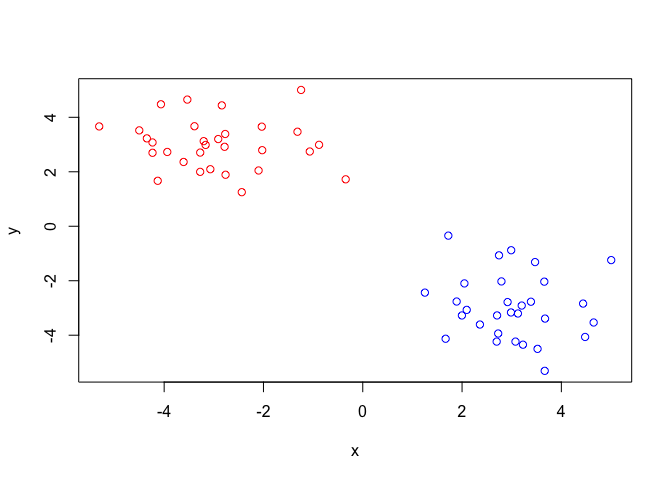
\includegraphics{class05_files/figure-latex/unnamed-chunk-5-1.pdf}

\section{?plot}\label{plot}

\begin{Shaded}
\begin{Highlighting}[]
\KeywordTok{plot}\NormalTok{(}\DecValTok{1}\NormalTok{:}\DecValTok{5}\NormalTok{, }\DataTypeTok{pch=}\DecValTok{1}\NormalTok{:}\DecValTok{5}\NormalTok{, }\DataTypeTok{cex=}\DecValTok{1}\NormalTok{:}\DecValTok{5}\NormalTok{, }\DataTypeTok{col=}\DecValTok{1}\NormalTok{:}\DecValTok{5}\NormalTok{)}
\end{Highlighting}
\end{Shaded}

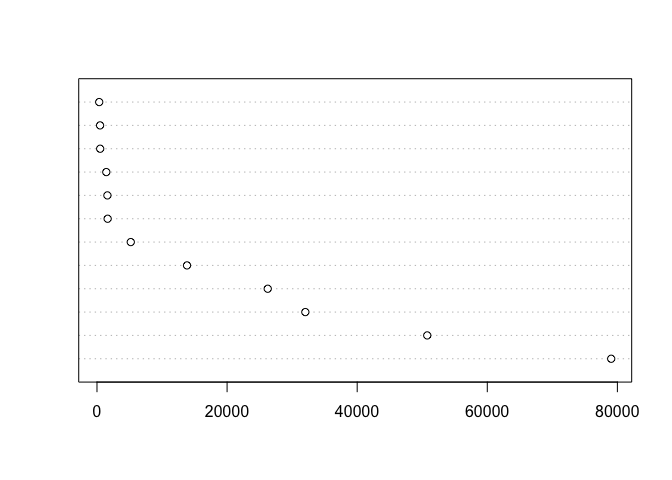
\includegraphics{class05_files/figure-latex/unnamed-chunk-6-1.pdf}

\begin{Shaded}
\begin{Highlighting}[]
\NormalTok{mouse <-}\StringTok{ }\KeywordTok{read.table}\NormalTok{(}\StringTok{"bimm143_05_rstats/feature_counts.txt"}\NormalTok{, }
                             \DataTypeTok{header =} \OtherTok{TRUE}\NormalTok{, }\DataTypeTok{sep =} \StringTok{"}\CharTok{\textbackslash{}t}\StringTok{"}\NormalTok{)}
\end{Highlighting}
\end{Shaded}

\begin{Shaded}
\begin{Highlighting}[]
\KeywordTok{dotchart}\NormalTok{(mouse$Count)}
\end{Highlighting}
\end{Shaded}

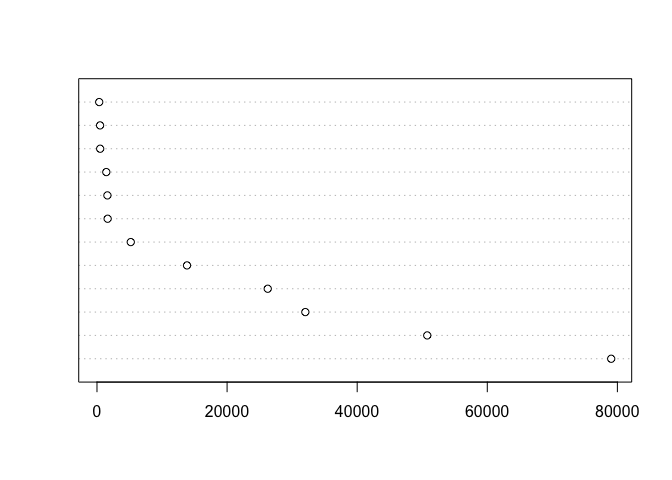
\includegraphics{class05_files/figure-latex/unnamed-chunk-8-1.pdf}

\section{?par()\$mar}\label{parmar}

\section{?barplot}\label{barplot}

\begin{Shaded}
\begin{Highlighting}[]
\KeywordTok{par}\NormalTok{(}\DataTypeTok{mar=}\KeywordTok{c}\NormalTok{(}\FloatTok{5.1}\NormalTok{, }\FloatTok{12.1}\NormalTok{, }\FloatTok{4.1}\NormalTok{, }\FloatTok{2.1}\NormalTok{))}
\KeywordTok{barplot}\NormalTok{(mouse$Count, }\DataTypeTok{horiz =} \OtherTok{TRUE}\NormalTok{, }\DataTypeTok{ylab=}\StringTok{""}\NormalTok{, }\DataTypeTok{names.arg =} \NormalTok{mouse$Feature, }
        \DataTypeTok{main=}\StringTok{"Mouse GRCm38 Genome Features"}\NormalTok{, }\DataTypeTok{las=}\DecValTok{1}\NormalTok{, }\DataTypeTok{xlim=}\KeywordTok{c}\NormalTok{(}\DecValTok{0}\NormalTok{,}\DecValTok{80000}\NormalTok{))}
\end{Highlighting}
\end{Shaded}

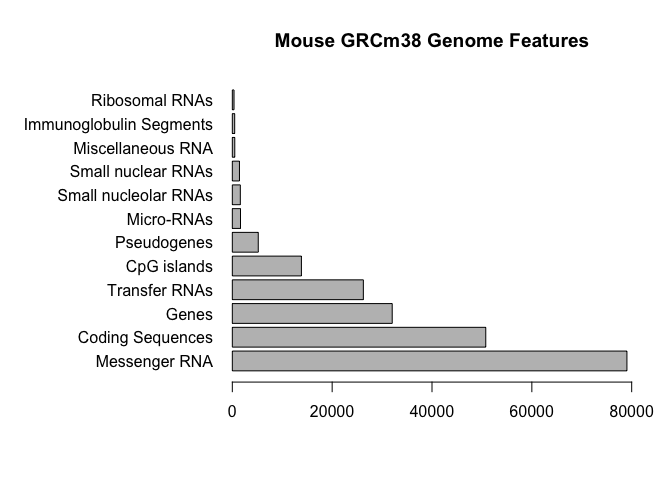
\includegraphics{class05_files/figure-latex/unnamed-chunk-9-1.pdf}

\begin{Shaded}
\begin{Highlighting}[]
\NormalTok{mf <-}\StringTok{ }\KeywordTok{read.delim}\NormalTok{(}\StringTok{"bimm143_05_rstats/male_female_counts.txt"}\NormalTok{)}
\KeywordTok{barplot}\NormalTok{(mf$Count, }\DataTypeTok{names.arg =} \NormalTok{mf$Sample, }\DataTypeTok{col=}\KeywordTok{rainbow}\NormalTok{(}\DecValTok{10}\NormalTok{))}
\end{Highlighting}
\end{Shaded}

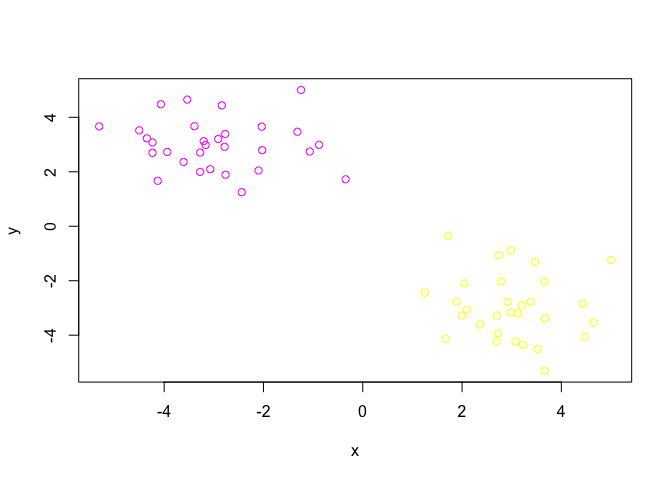
\includegraphics{class05_files/figure-latex/unnamed-chunk-10-1.pdf}

\begin{Shaded}
\begin{Highlighting}[]
\KeywordTok{rainbow}\NormalTok{(}\DecValTok{10}\NormalTok{)}
\end{Highlighting}
\end{Shaded}

\begin{verbatim}
##  [1] "#FF0000FF" "#FF9900FF" "#CCFF00FF" "#33FF00FF" "#00FF66FF" "#00FFFFFF"
##  [7] "#0066FFFF" "#3300FFFF" "#CC00FFFF" "#FF0099FF"
\end{verbatim}

\begin{Shaded}
\begin{Highlighting}[]
\NormalTok{mf <-}\StringTok{ }\KeywordTok{read.delim}\NormalTok{(}\StringTok{"bimm143_05_rstats/male_female_counts.txt"}\NormalTok{)}
\KeywordTok{barplot}\NormalTok{(mf$Count, }\DataTypeTok{names.arg =} \NormalTok{mf$Sample, }\DataTypeTok{col=}\KeywordTok{c}\NormalTok{(}\StringTok{"lightblue"}\NormalTok{, }\StringTok{"pink"}\NormalTok{), }\DataTypeTok{las=}\DecValTok{2}\NormalTok{)}
\end{Highlighting}
\end{Shaded}

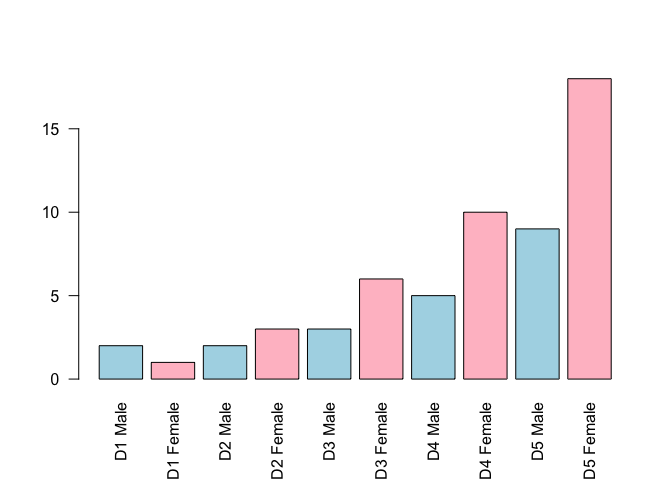
\includegraphics{class05_files/figure-latex/unnamed-chunk-12-1.pdf}

\begin{Shaded}
\begin{Highlighting}[]
\KeywordTok{barplot}\NormalTok{(mf$Count, }\DataTypeTok{names.arg=}\NormalTok{mf$Sample, }\DataTypeTok{col=}\KeywordTok{rainbow}\NormalTok{(}\KeywordTok{nrow}\NormalTok{(mf)))}
\end{Highlighting}
\end{Shaded}

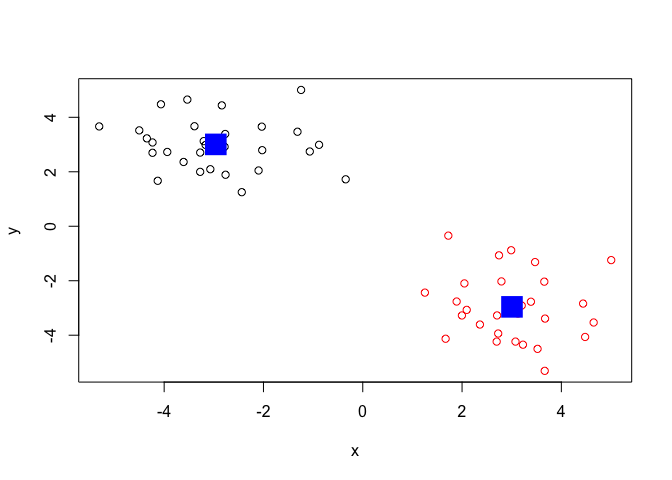
\includegraphics{class05_files/figure-latex/unnamed-chunk-13-1.pdf}

\end{document}
